\documentclass[letterpaper]{article}
\usepackage[margin=1in]{geometry}
\usepackage[utf8]{inputenc}
\usepackage{textcomp}
\usepackage{amssymb}
\usepackage{natbib}
\usepackage{graphicx}
\usepackage{gensymb}
\usepackage{amsthm, amsmath, mathtools}
\usepackage[dvipsnames]{xcolor}
\usepackage{enumerate}
\usepackage{mdframed}
\usepackage[most]{tcolorbox}
\usepackage{csquotes}
% https://tex.stackexchange.com/questions/13506/how-to-continue-the-framed-text-box-on-multiple-pages

\tcbuselibrary{theorems}

\newcommand{\R}{\mathbb{R}}
\newcommand{\Z}{\mathbb{Z}}
\newcommand{\N}{\mathbb{N}}
\newcommand{\Q}{\mathbb{Q}}
\newcommand{\C}{\mathbb{C}}
\newcommand{\code}[1]{\texttt{#1}}
\newcommand{\mdiamond}{$\diamondsuit$}
\newcommand{\PowerSet}{\mathcal{P}}
\newcommand{\Mod}[1]{\ (\mathrm{mod}\ #1)}
\DeclareMathOperator{\lcm}{lcm}

%\newtheorem*{theorem}{Theorem}
%\newtheorem*{definition}{Definition}
%\newtheorem*{corollary}{Corollary}
%\newtheorem*{lemma}{Lemma}
\newtheorem*{proposition}{Proposition}


\newtcbtheorem[number within=section]{theorem}{Theorem}
{colback=green!5,colframe=green!35!black,fonttitle=\bfseries}{th}

\newtcbtheorem[number within=section]{definition}{Definition}
{colback=blue!5,colframe=blue!35!black,fonttitle=\bfseries}{def}

\newtcbtheorem[number within=section]{corollary}{Corollary}
{colback=yellow!5,colframe=yellow!35!black,fonttitle=\bfseries}{cor}

\newtcbtheorem[number within=section]{lemma}{Lemma}
{colback=red!5,colframe=red!35!black,fonttitle=\bfseries}{lem}

\newtcbtheorem[number within=section]{example}{Example}
{colback=white!5,colframe=white!35!black,fonttitle=\bfseries}{def}

\newtcbtheorem[number within=section]{note}{Important Note}{
        enhanced,
        sharp corners,
        attach boxed title to top left={
            xshift=-1mm,
            yshift=-5mm,
            yshifttext=-1mm
        },
        top=1.5em,
        colback=white,
        colframe=black,
        fonttitle=\bfseries,
        boxed title style={
            sharp corners,
            size=small,
            colback=red!75!black,
            colframe=red!75!black,
        } 
    }{impnote}
\usepackage[utf8]{inputenc}
\usepackage[english]{babel}
\usepackage{fancyhdr}
\usepackage[hidelinks]{hyperref}

\pagestyle{fancy}
\fancyhf{}
\rhead{Math 170B}
\chead{Friday, April 28, 2023}
\lhead{Lecture 12}
\rfoot{\thepage}

\setlength{\parindent}{0pt}

\begin{document}

\section{Hermite Interpolation (Section 6.3)}
In Hermite interpolation, the derivatives are included in this interpolation condition. This is different from Lagrange interpolation, where derivatives aren't used. 

\bigskip 

Now, let's suppose we have $x_0, x_1$ with interpolation conditions such that \[P(x_i) = f(x_i), \quad P'(x_i) = f'(x_i), \quad i = 0, 1.\]
There are four\footnote{Note that $i = 0$, $i = 1$ are two conditions.} conditions in total. Thus, we want to seek polynomial of degree at most 3; in other words, we want to find 
\[P(x) = a + b(x - x_0) + c(x - x_0)^2 + d(x - x_0)^2 (x - x_1).\]
Finding the derivative, 
\[P'(x) = b + 2c(x - x_0) + 2d(x - x_0)(x - x_1) + d(x - x_0)^2.\]
Then, 
\[P(x_0) = a = f(x_0).\]
\[P'(x_0) = b = f'(x_0).\]
\[P(x_1) = a + b(x_1 - x_0) + c(x_1 - x_0)^2 = f(x_1).\]
\[P'(x_1) = b + 2c(x_1 - x_0) + d(x_1 - x_0)^2 = f'(x_1).\]
To simplify things, let $h = x_n - x_0$. Then, we can write out a matrix like so 
\[\begin{bmatrix}
    1 & 0 & 0 & 0 \\ 
    0 & 1 & 0 & 0 \\ 
    1 & h & h^2 & 0 \\ 
    0 & 1 & 2h & h^2
\end{bmatrix} \begin{bmatrix}
    a \\ 
    b \\ 
    c \\ 
    d 
\end{bmatrix} = \begin{bmatrix}
    f(x_0) \\ 
    f(x_1) \\ 
    f'(x_0) \\ 
    f'(x_1)
\end{bmatrix}.\]
In general, the system for solving these coefficients with derivative data does not have to be nonsingular. 

\subsection{Hermite Interpolation Conditions}
We need a condition to ensure that the polynomials can be found. In particular, this condition is related to the highest derivative that is included in the interpolation problem. So, for example, if at $x_0$ we want to interpolate at the third derivative, then the problem must also include the 0th, 1st, and 2nd derivatives. This can happen for a set of different $x$-values. Thus, the condition given is 
\[P^{(j)}(x_i) = \underbrace{c_{ij}}_{\text{Data}} \quad (0 \leq j \leq k_i - 1, 0 \leq i \leq m).\] 
Here, $k_i$ is the number of perscribed interpolatory conditions associated with the node $x_i$. 
So, the total condition is that 
\[k_0 + k_1 + \hdots + k_m \equiv m + 1.\]
So, the interpolating polynomial $P$ is of degree \emph{at most} $m$.

\begin{mdframed}[nobreak=true]
    (Example.) Suppose $m = 1$, $k_0 = 2$, $k_1 = 2$. Then, $m = 3$ since $k_0 + k_1 = 4 = 3 + 1 = m + 1$. With a polynomial of degree $m = 3$, for each $i$, the data that we need to have to get an interpolating polynomial is: 
    \begin{itemize}
        \item $i = 0$: $c_{00}, c_{01}$
        \item $i = 1$: $c_{10}, c_{11}$
    \end{itemize}
\end{mdframed}

\begin{mdframed}
    (Example.) Suppose we want to use Hermite Interpolation with just one point, $x_0$. Then, $i$ will be fixed at 0 but we can have $k$ derivatives. Thus, $p^{(j)}(x_0) = c_{0j}$ (where $c_{0j}$ is data that's given) for $0 \leq j \leq k$. The degree $k$ polynomial can fit this data: 
    \[P(x) = a_0 + a_1 (x - x_) + a_2 (x - x_0)^2 + \hdots + a_k (x - x_0)^k.\]
    Using $x = x_0$, we have 
    \[\begin{aligned}
        P(x_0) &= a_0 = c_{00} \\
        P'(x_0) &= a_1 = c_{01} \\ 
        &\vdots \\ 
        P^{(k)}(x_0) &= k! a_k = c_{0k}.
    \end{aligned}\]
    So, in particular, the coefficients are $a_0 = c_{00}$, $a_1 = c_{01} / 1$, and so on until $a_k = c_{0k} / k!$. Now, 
    \[P(x) = c_{00} + c_{01}(x - x_0) + \frac{c_{02}}{2!}(x - x_0)^2 + \hdots + \frac{c_{0k}}{k!}(x - x_0)^k.\]
\end{mdframed}

\subsection{Extended Divided Differences}
We can account for repeated modes, $x_i$, by creating the extended divided difference table. As is the case, the coefficients for each term of the interpolating polynomial will be in the first row of the table.
\begin{mdframed}
    (Example.) Suppose we are \emph{given} three data points, 
    \[P(x_0) = c_{00}, \quad P'(x_0) = c_{01}, \quad P(x_1) = c_{10}.\]
    We can create a divided difference table, shown below: 
    \begin{center}
        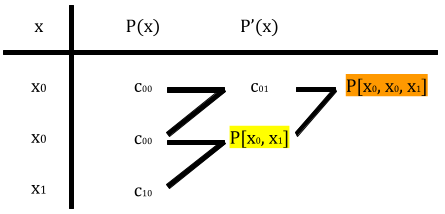
\includegraphics[scale=0.8]{../assets/hermite_example_ext.png}
    \end{center}

    Then, we find that 
    \[P[x_0, x_1] = \frac{P[x_1] - P[x_0]}{x_1 - x_0} = \frac{c_{10} - c_{00}}{x_1 - x_0}.\]
    \[P[x_0, x_0, x_1] = \frac{P[x_0, x_1] - P[x_0, x_0]}{x_1 - x_0} = \frac{\frac{c_{10} - c_{00}}{x_1 - x_0} - c_{01}}{x_1 - x_0}.\]
    Note that, for the denominator, we want the highest index minus the lowest index of the nodes. Then, we find that 
    \[P(x) = c_{00} + c_{01}(x - x_0) + P[x_0, x_0, x_1](x - x_0)^2.\]
\end{mdframed}

\end{document}